\appendix
\chapter{Vollständiges Boardlayout}\label{app:boardlayout}
\begin{figure}[H]%
\centering
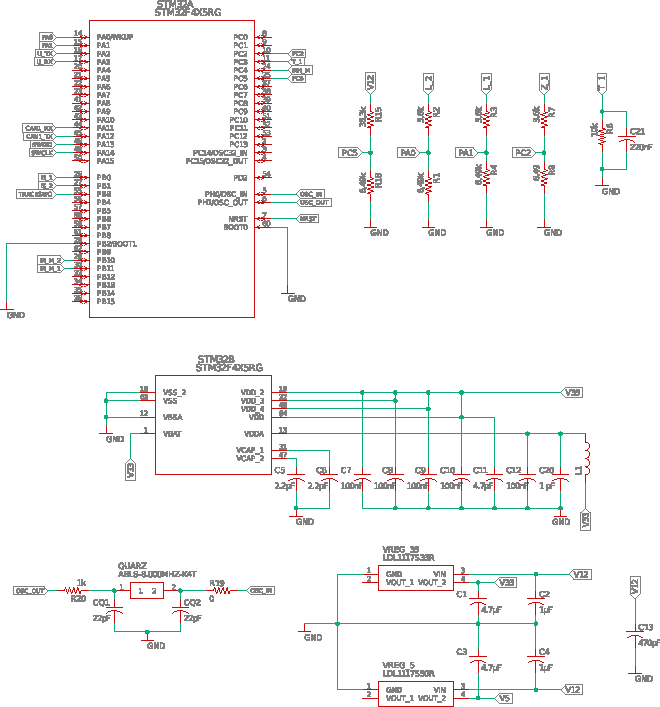
\includegraphics[angle=0,width=1
\columnwidth]{./Bilder/schem_app_1}%
\caption{Schaltplan MCU, Quarz, Spannungsregler, Spannungsteiler Sensorik}%
\label{}%
\end{figure}\newpage
\begin{figure}[H]%
\centering
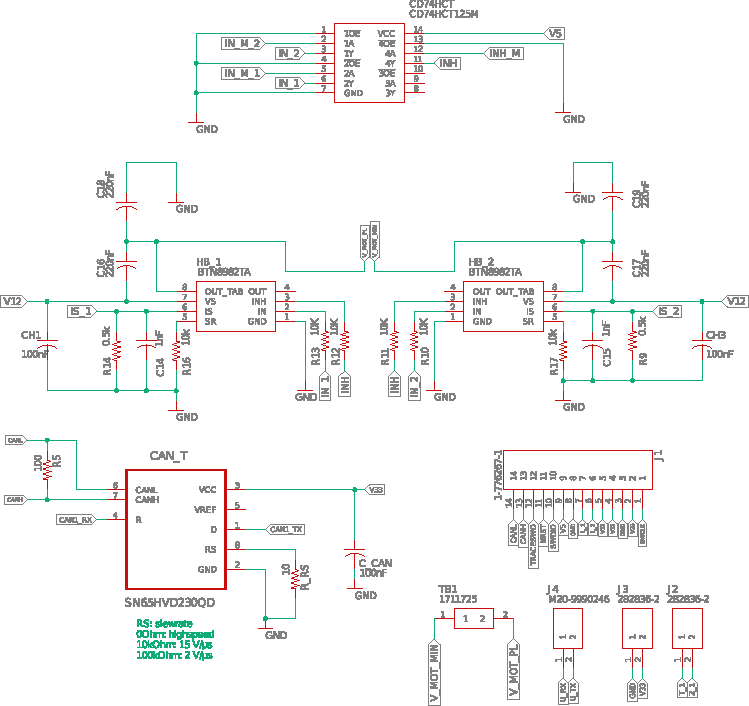
\includegraphics[angle=0,width=1
\columnwidth]{./Bilder/schem_app_2}%
\caption{Schaltplan CAN-Transciever, H-Brücke, Leitungstreiber, Ausgangsblöcke, Stecker}%
\label{}%
\end{figure}\newpage
\begin{figure}[H]%
\centering
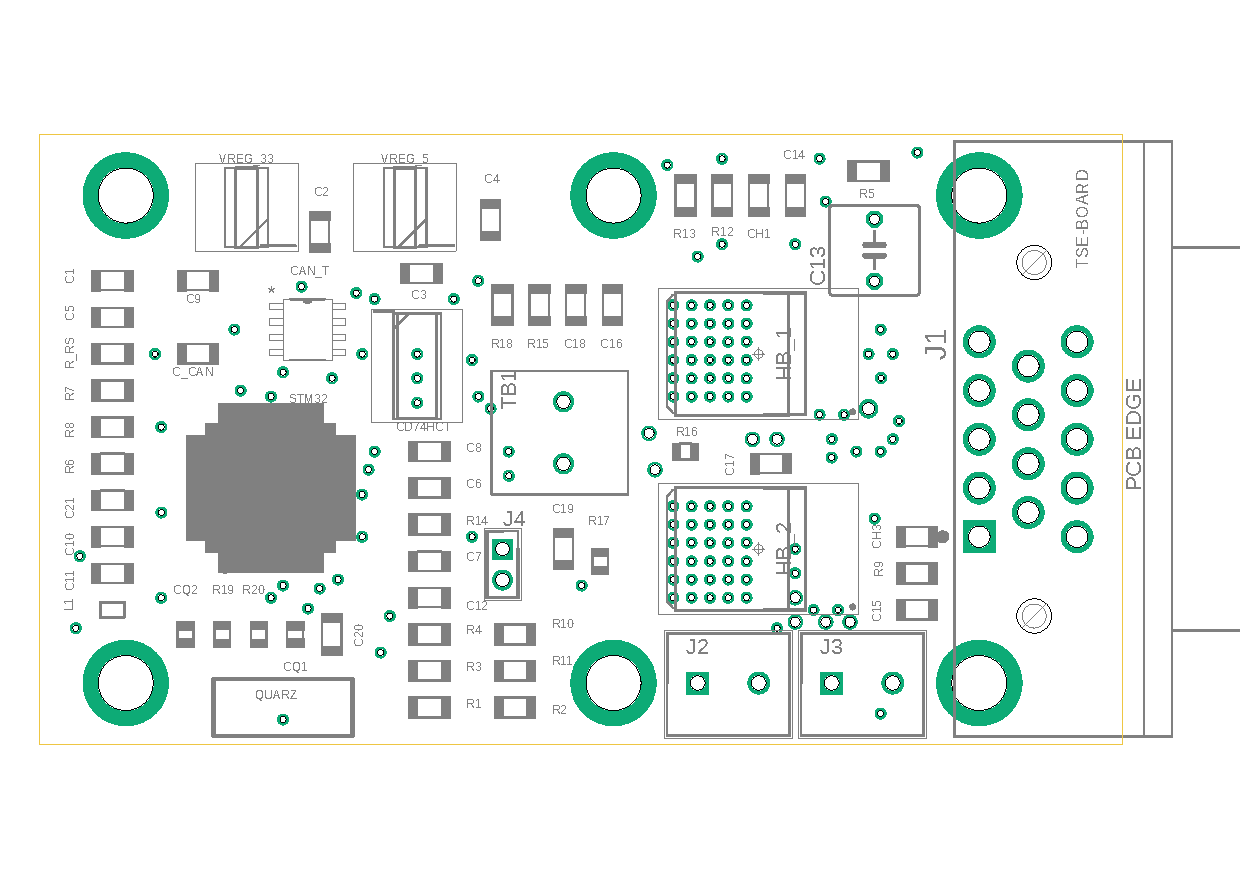
\includegraphics[angle=-90,width=0.7\columnwidth]{./Bilder/docu}%
\caption{Bauteilplatzierung des 2-Layer-Entwurfs}%
\label{}%
\end{figure}\newpage
\begin{figure}[H]%
\centering
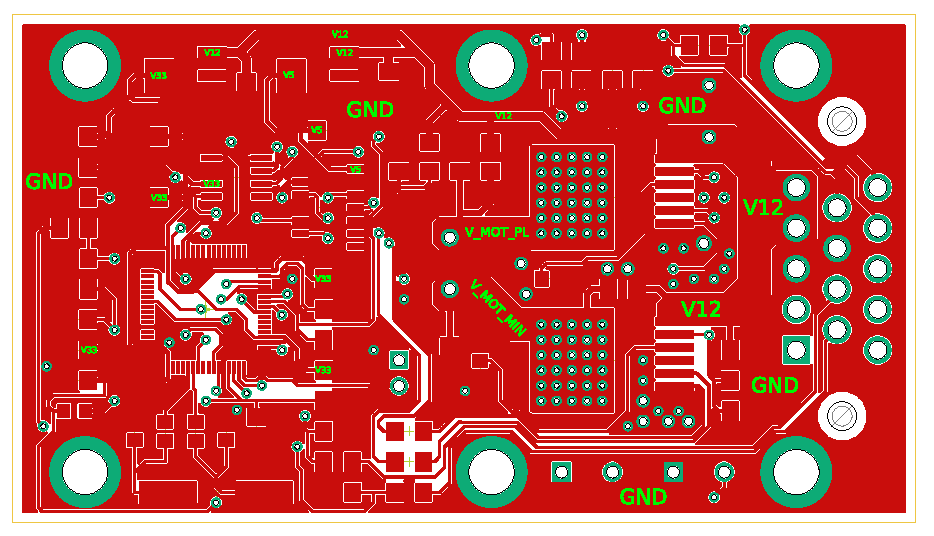
\includegraphics[angle=-90,width=0.7\columnwidth]{./Bilder/top2}%
\caption{Top-Layer des 2-Layer-Entwurfs}%
\label{}%
\end{figure}\newpage
\begin{figure}[H]%
\centering
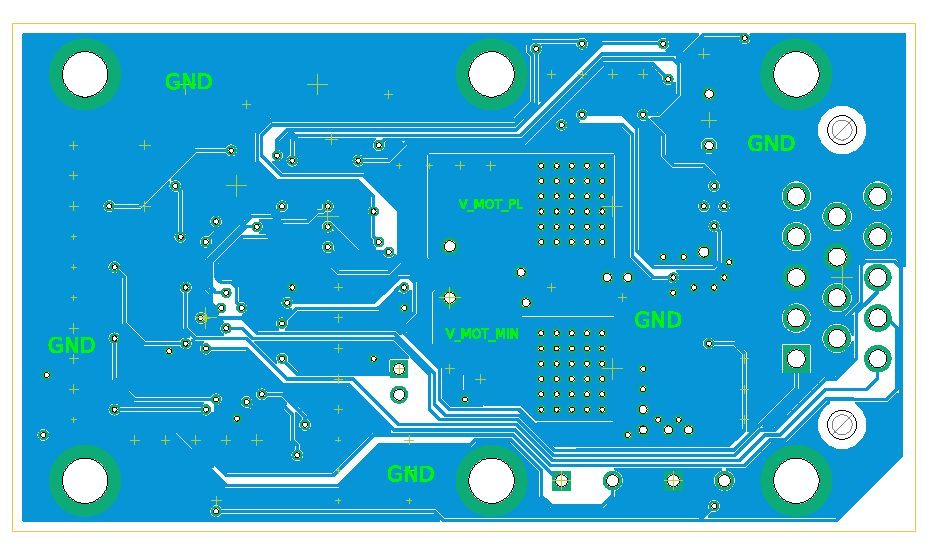
\includegraphics[angle=-90,width=0.7\columnwidth]{./Bilder/bottom2}%
\caption{Bottom-Layer des 2-Layer-Entwurfs}%
\label{}%
\end{figure}

\chapter{Alternativkonzept auf 4 Layern mit Buck-Converter}\label{app:4layer}
Wie in \autoref{sec:platan} beschrieben sind bisher keine Probleme durch EMI aufgetreten, sodass die Erweiterung auf ein 4-Layer Platinenlayout nur notwendig wäre, wenn in der zukünftigen Aktorkonfiguration Probleme auftreten sollen. Die Erweiterung bezieht sich hauptsächlich auf die Einführung eines Buck-Converters aus \autoref{fig:buckcon}, welcher die \SI{5}{V} Spannungsebene erzeugen könnte und die Einführung einer GND-Plane im zweiten Layer (vgl. \autoref{fig:groundplane}). Der Buck-Converter regelt auf die \SI{5}{V} über Schaltzyklen ähnlich denen eines PWM-Signals. Über die \SI{5}{V} des Buck-Converters wird der LDO für die \SI{3,3}{V} Spannungsebene gespeist, wie \autoref{fig:ldobuck} zeigt.
\begin{figure}[H]%
\centering
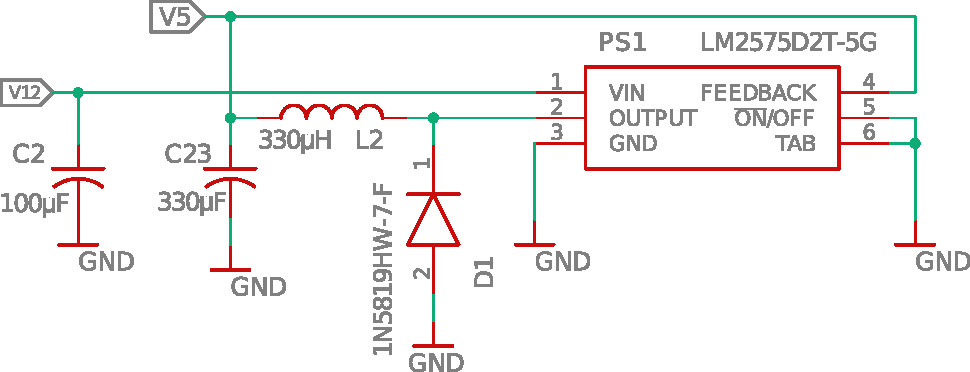
\includegraphics[width=0.8\columnwidth]{./Bilder/buck}%
\caption{Buck-Converter zum Regeln auf \SI{5}{V}}%
\label{fig:buckcon}%
\end{figure}\noindent
Diese Konfiguration hat den Vorteil, dass der LDO der \SI{3,3}{V} Spannungsebene weniger stark belastet wird. Problem an einem Buck-Converter ist, dass aufgrund der Schaltzyklen die Spannung weniger konstant ist, als bei einem LDO. Durch die Kombination beider Regler ist die \SI{3,3}{V} Spannungsebene so stabil wie in der vorherigen Spannungsregler-Konfiguration. Zu Analysieren wäre allerdings, wie sich der Buck-Converter auf das Auslesen der Lagesensorik auswirkt, welche von den \SI{5}{V} gespeist wird. Im derzeitigen Entwurf wurde sich deshalb für zwei seperate LDOs entschieden (vgl. \autoref{sec:spannver}).
\begin{figure}[H]%
\centering
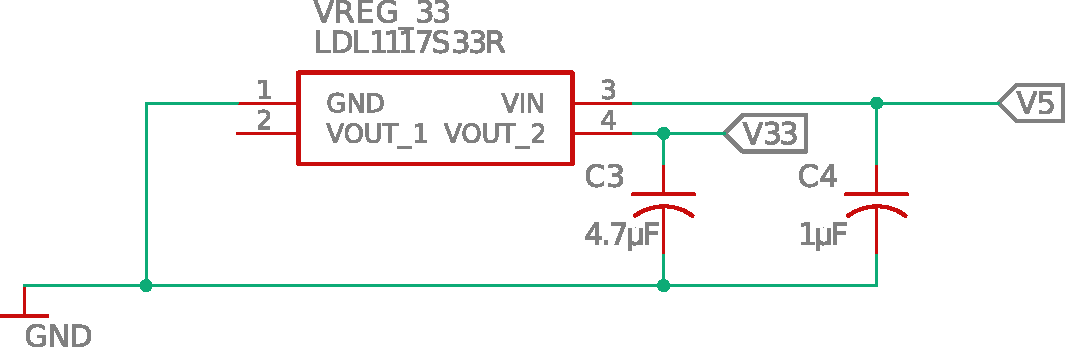
\includegraphics[width=0.8\columnwidth]{./Bilder/v334layer}%
\caption{LDO-Converter zum Regeln auf \SI{3,3}{V} bei \SI{5}{V} Eingangsspannung}%
\label{fig:ldobuck}%
\end{figure}\noindent
Nach \cite{Franz2012} wird die GND-Plane in Layer 2 (vgl. \autoref{fig:groundplane}) eingeführt um eine Abschirmung des Top-Layers gegenüber Layer 3 und Layer 4 zu erreichen, was eine Verbesserung der EMV bezweckt. Die Signalleitungen werden so möglichst in den unteren Layern verlegt um eine gute Abschirmung zu garantieren \cite{emcdes}.
\newpage
\begin{figure}[H]%
\centering
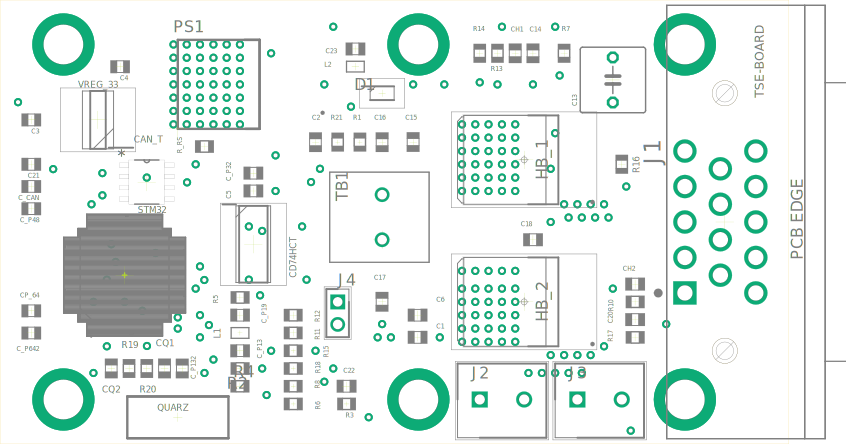
\includegraphics[angle=-90,width=0.7\columnwidth]{./Bilder/doc4layer}%
\caption{Bauteilplatzierung des 4-Layer-Entwurfs}%
\label{}%
\end{figure}\newpage
\begin{figure}[H]%
\centering
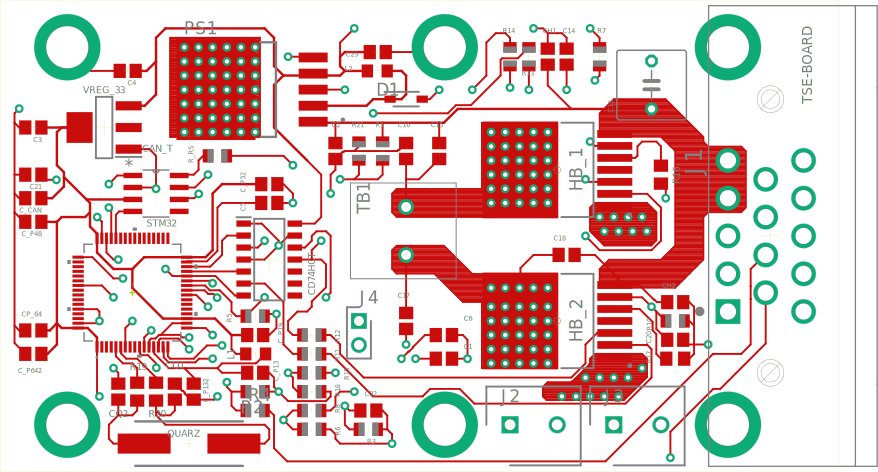
\includegraphics[angle=-90,width=0.7\columnwidth]{./Bilder/top4layer}%
\caption{Top-Layer des 4-Layer-Entwurfs}%
\label{}%
\end{figure}\newpage
\begin{figure}[H]%
\centering
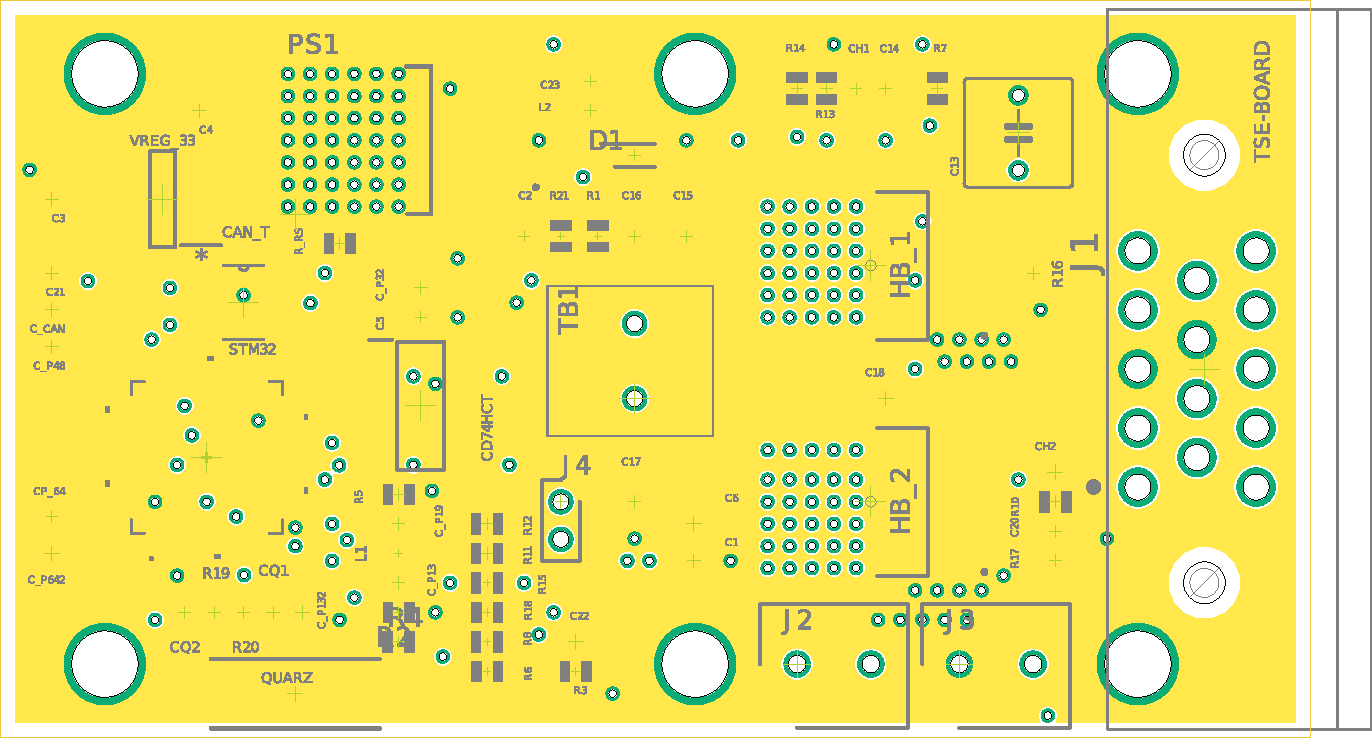
\includegraphics[angle=-90,width=0.7\columnwidth]{./Bilder/2route4layer}%
\caption{Zweites Layer des 4-Layer-Entwurfs}%
\label{fig:groundplane}%
\end{figure}\newpage
\begin{figure}[H]%
\centering
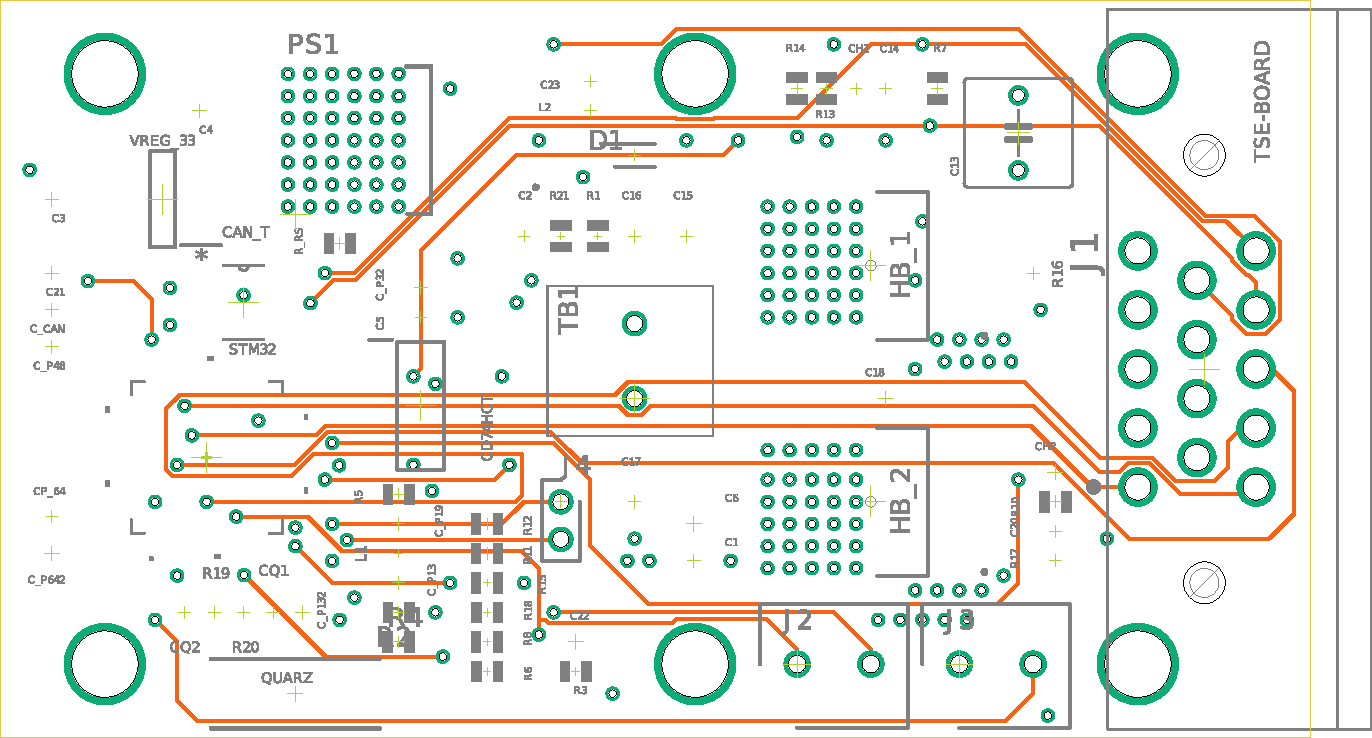
\includegraphics[angle=-90,width=0.7\columnwidth]{./Bilder/15route4layer}%
\caption{Drittes Layer des 4-Layer-Entwurfs}%
\label{}%
\end{figure}\newpage
\begin{figure}[H]%
\centering
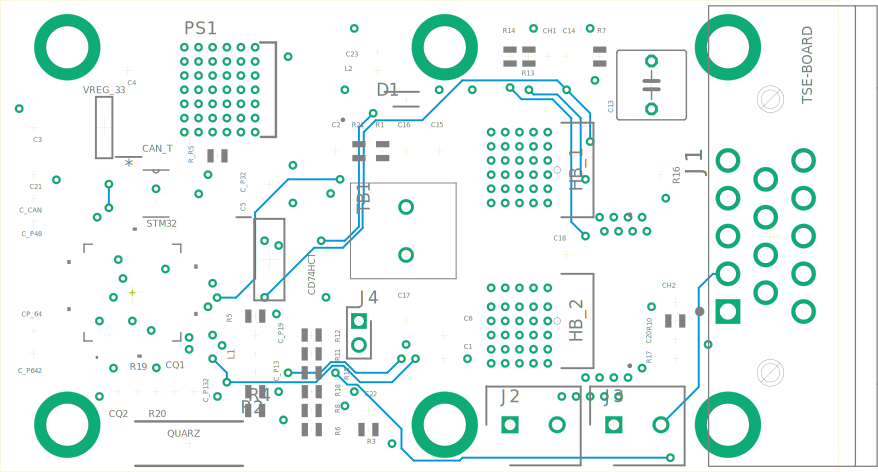
\includegraphics[angle=-90,width=0.7\columnwidth]{./Bilder/bot4layer}%
\caption{Bottom-Layer des 4-Layer-Entwurfs}%
\label{}%
\end{figure}
\cleardoublepage
\chapter{Datenblätter}
\section{Auszug aus den EMC Design Guidelines von Infineon - AP24026}
\begin{center}
	
\includegraphics[page=17,width=0.85\columnwidth]{./datenblaetter/infineon_design}
\end{center}
\section{Auszug aus dem Oscillator Design Guide for STM32 von STMicroelectronics - AN2867}
\begin{center}
	\includegraphics[page=31,width=0.96\columnwidth]{./datenblaetter/quarzinfo_stm}
\end{center}
\section{Auszug aus dem User Manual des ST-LINK/V2 von STMicroelectronics - UM1075}
\begin{center}\label{app:stlink}
	\includegraphics[page=12,width=0.96\columnwidth]{./datenblaetter/ST_LINK_V2}
\end{center}
\section{Auszug aus der Application Note Using Decoupling Capacitors von Cypress - AN1032}
\begin{center}
	\includegraphics[page=3,width=0.96\columnwidth]{./datenblaetter/decoupling}
\end{center}
\section{Auszug aus dem Datenblatt des STM32F405xx, STM2F407xx}\label{app:stm32man}
\begin{center}
	\includegraphics[page=77,width=0.98\columnwidth]{./datenblaetter/STM32F407_MC}
\end{center}
\section{Auszug aus IPC-2221 - Generic Standard on
Printed Board Design}
\begin{center} \label{app:ipc}
	
\includegraphics[page=50,width=0.98\columnwidth]{./datenblaetter/IPC-2221-2}
\end{center}